%============================================================
\section{Nombre: Ventisca.} \label{ventisca}
\subsection{Descripción}
El enemigo dispara una secuencia de cristales de hielo de manera repetida durante un periodo de tiempo. El disparo de estos cristales se dará en la dirección hacia la que este mirando el enemigo. Cada cristal reduce la cantidad de vida del jugador al colisionar con él. Los cristales se destruirán al colisionar con otro objeto que no sea el jugador o después de un tiempo si no han colisionado con ningún objeto.
\subsection{Portador}
Mictlecayotl (ver apartado \ref{per:mictlecayotl}).
\subsection{Esquema}
			Ver figura \ref{fig:ventisca}.
			\begin{figure}
				\centering
				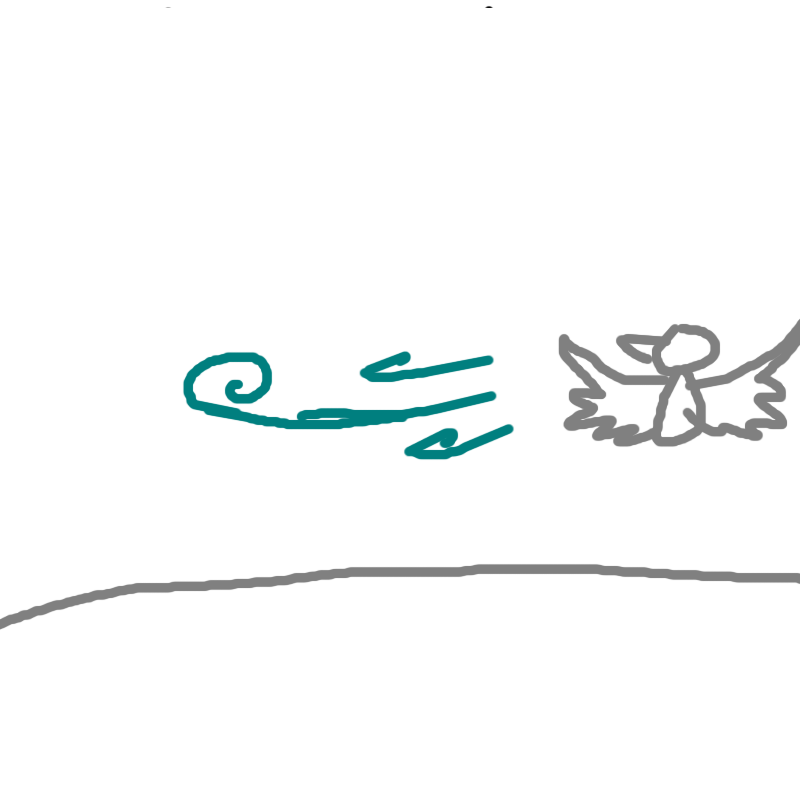
\includegraphics[height=0.2 \textheight]{Imagenes/ventisca}
				\caption{Ventisca.}
				\label{fig:ventisca}
			\end{figure}